
\chapter{Applicazione dei metodi alle simulazioni multibody}
In questo capitolo si vedrà come applicare i metodi numerici visti nel capitolo \ref{chap:cauchy} alle simulazioni multibody.

Si noti che nella definizione del problema di Cauchy (eq. \ref{eq:cauchy_def}) la funzione $f(t, y(t))$ viene considerata assegnata. Questo non accade in una simulazione, dal momento che lo stato del sistema non è noto a priori. \newline
Si consideri il sistema \ref{eq:dyn_sys}: la matrice dei coefficienti ed il vettore dei termini noti dipendono dallo stato futuro, e non è pertanto possibile calcolare direttamente $\avect{\Ddot{q}}$ e $\avect{\lambda}$ nel timestep futuro $t+1$ come richiesto dai metodi impliciti. \newline A questi algoritmi andrà pertanto abbinato il metodo di Newton per i sistemi.


\section{Cenni al metodo di Newton-Raphson o Metodo delle Tangenti}
\subsection{Metodo di Newton per la soluzione di equazioni non lineari}
Il metodo di Newton \cite{Quarteroni} può essere utilizzato per approssimare numericamente gli zeri di una funzione di una variabile reale, ossia data \(f:\mathbb{R} \rightarrow \mathbb{R}\) si cerca $\alpha\in \mathbb{C}\quad t.c.\quad f(\alpha)=0 $ \newline
Se $f \in C^1([a,b])\quad con \quad [a,b]\subset\mathbb{R} \quad t.c. \quad f(a)f(b) < 0 \quad e \quad f'(x) \neq 0 \forall x \in [a,b]$ si può procedere iterativamente al calcolo della radice una volta assegnato il valore iniziale $x^{0}$:
\begin{equation} \label{eq:Newton_1d}
    x^{(k+1)} = x^{(k)} - \frac{f\left(x^{(k)}\right)}{f'\left(x^{(k)}\right)}
\end{equation}
Sebbene il metodo richieda 2 valutazioni funzionali controbilancia l'onere computazionale con un ordine di convergenza 2 (quando la radice è semplice).
\begin{figure}[h!]
\centering
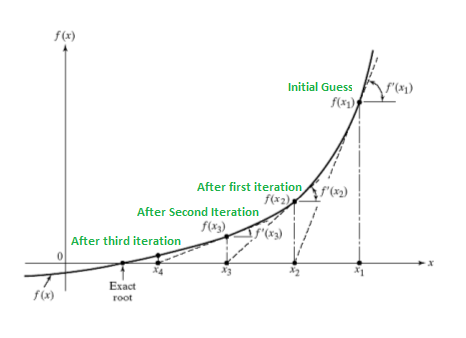
\includegraphics[height=8cm]{newtonRaphsonMethod.png}
\caption{Rappresentazione grafica per i passi del metodo di Newton}
 \label{fig:Newton_1d}
\end{figure}
\subsection{Metodo di Newton per la soluzione di sistemi}
Il metodo di Newton può essere esteso al caso di sistemi di equazioni. 
Il metodo può essere esteso al caso di sistemi di equazioni. Indicando con l'apice n l' n-esimo passaggio, con $\amatr{F}$ il sistema di equazioni e con $\amatr{J}$ il jacobiano di quest'ultimo si procede dato $\avect{x}{(0)}$ come segue:
\begin{align} \label{eq:NewtonRaphsonA}
    \amatr{J}\left( \avect{x}^{(n)} \right) \avect{\delta x}^{(n)} = - \amatr{F}\left( \avect{x}^{(n)} \right) \\
    \label{eq:NewtonRaphsonB}  \avect{x}^{(n+1)} = \avect{x}^{(n)} + \avect{\delta x}^{(n)} 
\end{align}
L'onere computazionale di questo metodo consiste nel risolvere ad ogni passaggio un sistema lineare di matrice $\amatr{J}$.

\section{Smorzamento Numerico} \label{sec_numdamp}
Lo smorzamento numerico (\textit{numerical damping}) indica un errore numerico, che si manifesta come la comparsa di uno smorzamento fittizio, tipica dei metodi impliciti ed, in taluni casi, semi-impliciti. Questo fenomeno è ben osservabile in un sistema massa-molla senza smorzatore, le cui oscillazioni dovrebbero mantenersi ad ampiezza costante, mentre diminuiscono nel tempo. Questo fenomeno si accentua al diradarsi del \textit{timestep}.
\subsection{Esempio numerico: smorzamento numerico in un sistema massa-molla implementato in Matlab}
Per osservare quanto affermato si riporta un esempio numerico del sistema massa molla. Con la solita notazione possiamo scrivere :\[\begin{cases}\frac{v^{l+1}-v^l}{h}M = f^{l+1}\\ q^{l+1}= q^l+v^{l+1}h \end{cases}\]
Nel caso del sistema massa-molla si avrà : \[f^l = Mg-Kq^l \]O, in presenza di smorzatore \[ f^l = Mg-Kq^l-Cv^l\]
Da cui:  \[ \left(v^{l+1}-v^l\right)M = h\left(  Mg-Kq^{l+1} -Cv^{l+1} \right)  \]
Sostituendo il valore di $q^{+1}$ si ottiene:
\[ \left(v^{l+1}-v^l\right)M = h\left(  Mg-K(q^l+v^{l+1}h) -Cv^{l+1} \right)  \]
Si può quindi scrivere:
\[ v^{l+1}\left(M+Kh^2+Ch\right) = Mv^l + h\left(  Mg-Kq^l \right)  \]
Possiamo quindi esprimere $v^{l+1}$
\[ v^{l+1} = \frac{ Mv^l + Mgh -Khq^l }{\left(M+Kh^2+Ch\right)}  \]
A questo punto si procede ad implementare in Matlab un algoritmo che risolve numericamente il sistema con \textit{timestep} crescente così da poter osservare l'andamento della smorzamento numerico. Si riporta la porzione di codice più significativa, ovvero il ciclo \textit{while} che calcola velocità e posizione nell'istante successivo e le memorizza.


\noindent\rule{\textwidth}{1pt}\newline  $ 
    while \  t<= Tmax \\
        vl1 = (m*v+m*g*dt-k*x*dt)/(m+k*dt^2+c*dt); \\
        xl1 = x + dt*vl1; \\
        t = t+ dt; \\
        v = vl1; \\
        x = xl1; \\
        j = j+1; \\
        v_{vett}(j) = vl1; \\
        x_{vett}(j) = xl1; \\
        t_{vett}(j) = t; \\
    end$ \newline
\noindent\rule{\textwidth}{1pt}
Di seguito sono riportati i grafici di spostamento e velocità della simulazione del sistema massa-molla che utilizza il loop riportato. Sebbene sia presente un termine di smorzamento esso è in realtà nullo. 

\begin{figure}[ht]
\centering
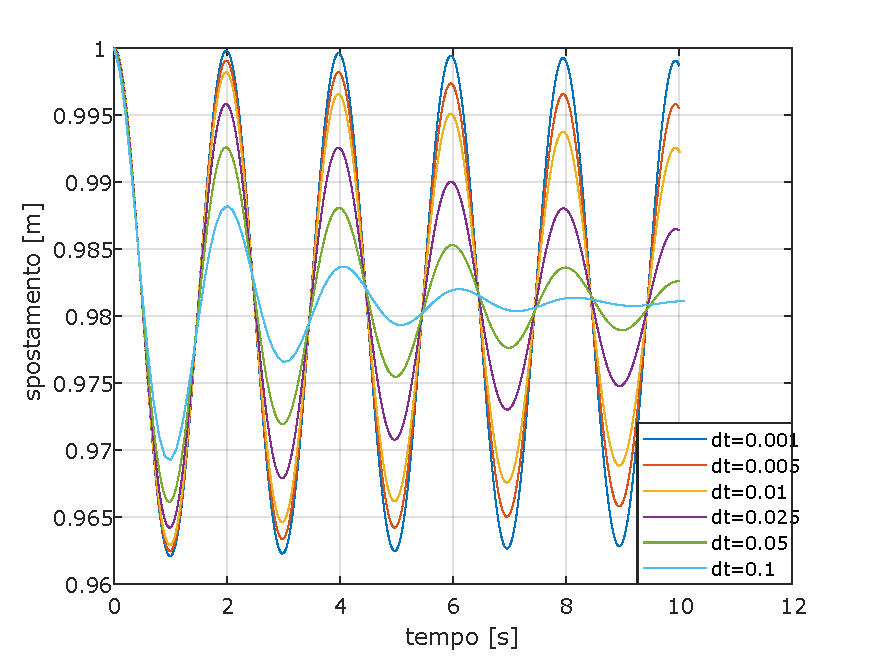
\includegraphics[height=5cm]{Figure/position.pdf}
\caption{Posizione della massa nel sistema massa-molla in funzione del tempo al variare del timestep}
 \label{fig:Newton_1d}
\end{figure}

\begin{figure}[h!]
\centering
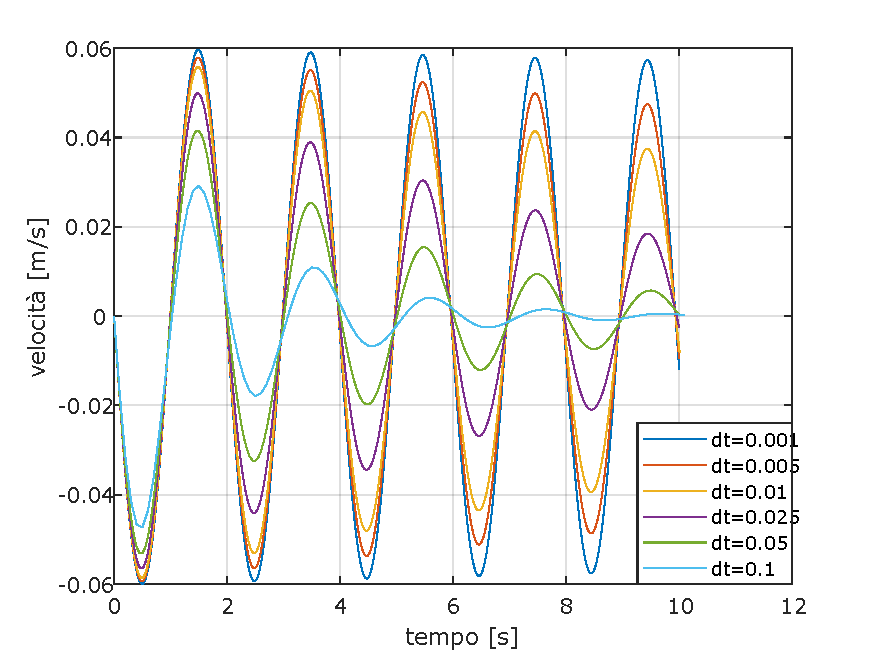
\includegraphics[height=5cm]{Figure/speed.pdf}
\caption{Velocità della massa nel sistema massa-molla in funzione del tempo al variare del timestep}
 \label{fig:Newton_1d}
\end{figure}

Ciononostante si nota una progressiva diminuzione dell'ampiezza delle oscillazioni, più accentuata all'aumentare del \textit{timestep}, mentre in condizioni di smorzamento nullo la soluzione analitica prevederebbe oscillazioni ad ampiezza costante. 

Lo smorzamento fittizio (in quanto derivato da un errore numerico e senza alcun riscontro fisico) osservabile è la manifestazione dello smorzamento numerico in questione. Infatti l'unica differenza tra le soluzioni è il progressivo aumento del \textit{timestep}.


\section{Algoritmi di soluzione per metodi impliciti}
\paragraph{Eulero implicito}
Di seguito si illustra l'applicazione del metodo di integrazione di Eulero implicito (Backward Euler) ad un sistema multibody in presenza di vicoli.
Si riprende l'equazione \ref{eq:dyn_sys}. Come accennato in precedenza non è possibile conoscere direttamente il valore delle forze nello stato $l+1$. Per pervenire ad una soluzione è necessario includere l'integrazione numerica all'interno di un'iterazione di Newton-Raphson.

Per un sistema multibody il metodo di Eulero implicito può essere scritto come il seguente sistema che chiameremo \textbf{G}
\begin{align} \label{eq:eulforw_Gq}
    \avect{q}^{l+1}-\avect{q}^l - \avect{v}^{l+1}h &= 0 \\ \label{eq:eulforw_Gv}
    \amatr{M}(\avect{v}^{l+1} -\avect{v}) - h\avect{f}^{l+1} - h\amatr{C}_q^T \avect{\lambda}^{l+1} &= 0 \\ \label{eq:eulforw_Glam}
    \amatr{C}(\avect{q}^{l+1} , t^{l+1}) &= 0
\end{align}
Per procedere alla soluzione iterativa con Newton come anticipato si deve esprimere lo Jacobiano del sistema \textbf{G}:
\begin{equation} \label{eq:eulforwjacob} \amatr{J} =
    \begin{bmatrix} I & -hI   & 0 \\
    -h\nabla_q\avect{f}^{l+1} & \amatr{M}-h\nabla_v\avect{f}^{l+1} &  -h\amatr{C}_q^T \\
    \amatr{C}_q               &  0                                 &    0  \end{bmatrix}
\end{equation}
Utilizzando il procedimento illustrato in \ref{eq:NewtonRaphsonA} si scrive:
\begin{equation} \label{eq:eulforw_iterstep}
    \amatr{J} \left\{\begin{array}{c}\Delta\avect{q}^{l+1} \\ \Delta\avect{v}^{l+1} 
    \\ \Delta\avect{\lambda}^{l+1} \end{array} \right\} = -\amatr{G} \end{equation}
Dalla prima riga dell'equazione \ref{eq:eulforw_iterstep}:
\[ \Delta\avect{q}^{l+1} = h\Delta\avect{v}^{l+1} -\avect{q}^{+1} +\avect{q}^l + h\avect{v}^{l+1} \]
E, differenziando l'equazione \ref{eq:eulforw_Gq} si ottiene 
\begin{equation}
    \Delta \avect{q}^{l+1} = h \Delta \avect{v}^{l+1}
\end{equation}

Questa approssimazione è vera solo in prossimità della soluzione ma viene comunemente usata per evitare la complicazione che proviene dal considerare tutti i termini del sistema.
Grazie a questa relazione possiamo eliminare la dipendenza di $\avect{q}^{l+1}$ da $\Delta \avect{q}^{l+1}$, infatti la prima equazione di \ref{eq:eulforw_iterstep} si semplifica divenendo identica alla \ref{eq:eulforw_Gq} e il sistema \ref{eq:eulforw_iterstep} diventa: 

\begin{equation}
        \begin{bmatrix} I & -hI   & 0 \\
    -h\nabla_q\avect{f}^{l+1} & \amatr{M}-h\nabla_v\avect{f}^{l+1} &  -h\amatr{C}_q^T \\
    \amatr{C}_q               &  0                                 &    0  \end{bmatrix}
    \left\{\begin{array}{c}h\Delta\avect{v}^{l+1} \\ \Delta\avect{v}^{l+1} 
    \\ \Delta\avect{\lambda}^{l+1} \end{array} \right\}
    = -\amatr{G}
\end{equation}
La seconda e terza equazione possono essere riscritte come segue, la prima è riportata in fondo e vengono aggiunti i passaggi del procedimento di Newton Raphson \ref{eq:NewtonRaphsonB} per $v$ d $\lambda$.
\[
    \begin{bmatrix}\left[ M-h^2\nabla_q\avect{f}^{l+1}-h\nabla_v\avect{f}^{l+1} \right] & \amatr{C}_q^T \\\amatr{C}_q &0 \end{bmatrix} \left\{\begin{array}{c} \Delta\avect{v}^{l+1}  \\ 
    -h\Delta\avect{\lambda}^{l+1} \end{array} \right\} = \] \begin{equation} \label{eq:eulfor_NRiter1} =
    \left\{\begin{array}{c} (\avect{v}^l-\avect{v}^{l+1})\amatr{M}+h\avect{f}^{l+1}+h\amatr{C}_q^T \avect{\lambda}^{l+1}\\ -\frac{\amatr{C^{l+1}}}{h} \end{array} \right\}
\end{equation}
\begin{equation}
        \avect{v}_{n+1}^{l+1} = \avect{v}_n^{l+1} + \Delta\avect{v}^{l+1}
\end{equation}
\begin{equation}
        \avect{\lambda}_{n+1}^{l+1} = \avect{\lambda}_n^{l+1} + \Delta\avect{\lambda}^{l+1}
\end{equation}
\begin{equation} \label{eq:eulfor_NRiter4}
        \avect{q}^{l+1} = \avect{q}^l + h\avect{v}_{n+1}^{l+1}
\end{equation}
Si noti che \begin{itemize}
    \item L'indice dell'iterazione è passato al pedice in quanto l'apice è già utilizzato per indicare il timestep.
    \item $\avect{q}$ non dipende da $\Delta\avect{q}$ ma viene calcolato direttamente dato il valore aggiornato di $\avect{v}^{l+1}$ come espresso in \ref{eq:eulfor_NRiter4}
    \item Nella seconda equazione del sistema \ref{eq:eulfor_NRiter1} sono stati divisi entrambi i membri per $h$
\end{itemize}    
Questi passaggi sono implementati nel solver di Chrono e verranno analizzati nel seguente capitolo i dettagli implementativi.

\paragraph{Metodo dei trapezi }
Il procedimento è analogo a quanto visto per il metodo di Eulero, e la stessa cosa può essere detta per i metodi illustrati in seguito. Le differenze risiedono ovviamente nella definizione degli step di integrazione dando luogo a differenze nel sistema da implementare. Nello specifico il nuovo sistema \textbf{G} diventa:
\begin{align} \label{eq:trap_Gq}
    \avect{q}^{l+1}-\avect{q}^l - \frac{\avect{v}^{l+1}-\avect{v}^l}{2} h &= 0 \\ \label{eq:trap_Gv}
    \amatr{M}(\avect{v}^{l+1} -\avect{v}) - \frac{h}{2}(\avect{f}^{l+1} + \avect{f}^l )
    - \frac{h}{2}({\amatr{C}_q^{l+1}}^T \avect{\lambda}^{l+1} + {\amatr{C}_q^l}^T \avect{\lambda}^l) &= 0 \\ \label{eq:trap_Glam} \amatr{C}(\avect{q}^{l+1} , t^{l+1}) &= 0
\end{align}
Mentre in questo caso si avrà:
\begin{equation}
    \Delta \avect{q}^{l+1} = \frac{h}{2} \Delta \avect{v}^{l+1}
\end{equation}

Seguendo i passaggi effettuati per il metodo di Eulero:

\begin{align} \nonumber
\amatr{J} \left\{\begin{array}{c}\Delta\avect{q}^{l+1} \\ \Delta\avect{v}^{l+1}  
        \\ \Delta\avect{\lambda}^{l+1} \end{array} \right\} = -\amatr{G}
\\
\begin{bmatrix} I & -\frac{h}{2}I   & 0 \\
-\frac{h}{2}\nabla_q\avect{f}^{l+1} & \amatr{M}-\frac{h}{2}\nabla_v\avect{f}^{l+1} &-\frac{h}{2}\amatr{C}_q^T \\
    \amatr{C}_q^{l+1}              &  0                                 &    0  \end{bmatrix}
    \left\{\begin{array}{c}\frac{h}{2}\Delta\avect{v}^{l+1} \\ \Delta\avect{v}^{l+1} 
    \\ \Delta\avect{\lambda}^{l+1} \end{array} \right\}
    = - \amatr{G}
\end{align}
Da cui, sviluppando i calcoli ed aggiungendo gli incrementi di $\avect{v}$ e $\avect{\lambda}$:

\[
    \begin{bmatrix}\left[ M-\frac{h^2}{4}\nabla_q\avect{f}^{l+1}-\frac{h}{2}\nabla_v\avect{f}^{l+1} \right] 
    & {\amatr{C}_q^{l+1}}^T \\ \amatr{C}_q^{l+1} & 0 \end{bmatrix} 
    \left\{\begin{array}{c} \Delta\avect{v}^{l+1} \\ -\frac{h}{2}\Delta\avect{\lambda}^{l+1} \end{array}\right\}=\] 
    \begin{equation} \label{eq:eulfor_NRiter1} =
    \left\{\begin{array}{c} (\avect{v}^l-\avect{v}^{l+1})\amatr{M}+\frac{h}{2}(\avect{f}^{l+1} + \avect{f}^l {\amatr{C}_q^{l+1}}^T \avect{\lambda}^{l+1} + {\amatr{C}_q^l}^T \avect{\lambda}^l)\\ -\frac{\amatr{C^{l+1}}}{h} \end{array} \right\}
\end{equation}
\begin{equation}
        \avect{v}_{n+1}^{l+1} = \avect{v}_n^{l+1} + \Delta\avect{v}^{l+1}
\end{equation}
\begin{equation}
        \avect{\lambda}_{n+1}^{l+1} = \avect{\lambda}_n^{l+1} + \Delta\avect{\lambda}^{l+1}
\end{equation}
\begin{equation} \label{eq:eulfor_NRiter4}
        \avect{q}^{l+1} = \avect{q}^l + \frac{h}{2}(\avect{v}^l+\avect{v}_{n+1}^{l+1})
\end{equation}

\paragraph{Newmark}

Procedendo similmente a quanto visto nei casi precedenti si può scrivere \cite{negrutGavrea2005}:
\begin{align} \nonumber
    \begin{bmatrix}
    \amatr{H} & \overline{\amatr{C}_q}^T \\ \overline{\amatr{C}_q} & 0 
    \end{bmatrix}
    \begin{Bmatrix}
    \Delta \avect{a}^{l+1} \\ \Delta \avect{\lambda}^{l+1}
    \end{Bmatrix}  = \\
    \begin{Bmatrix}
        \amatr{M} \avect{a}^{l+1} - (\amatr{C}_q^T \avect{\lambda}+\avect{f})^{l+1} \\
        -\frac{1}{\beta h^2}\avect{C}^{l+1}
    \end{Bmatrix} \\
    \avect{a}_{n+1}^{l+1} = \avect{a}_n^{l+1} + \Delta a^{l+1} \\
    \avect{\lambda}_{n+1}^{l+1} = \avect{\lambda}_n^{l+1} + \Delta \lambda^{l+1} \\
    \avect{v}^{l+1} = \avect{v}^l +h \left[ (1-\gamma)\avect{a}^l + \gamma \avect{a}^{l+1} \right] \\
    \avect{q}^{l+1} = \avect{q}^l +h\avect{v}^l+\frac{h^2}{2}[(1-2\beta)\avect{a}^l+2\beta\avect{a}^{l+1}]
\end{align}
Dove $\amatr{H}$  è una matrice che raccoglie vari termini:
\begin{equation}
    \amatr{H} = \left[ \amatr{M}-\gamma h \nabla_v\avect{f}^{l+1} -\beta h^2 \nabla_q\avect{f}^{l+1} +
    \beta h^2 \left[ (\amatr{M} \avect{a})_q + (\amatr{C}_q^T \avect{\lambda})_q \right] \right]
\end{equation}

\paragraph{HHT} 
Per il metodo HHT \cite{Wang15HHT} \cite{JayNegrut2007}, invece, si ottiene:

\begin{align} \nonumber
    \begin{bmatrix}
    \amatr{H} & \overline{\amatr{C}_q}^T \\ \overline{\amatr{C}_q} & 0 
    \end{bmatrix}
    \begin{Bmatrix}
    \Delta \avect{a}^{l+1} \\ \Delta \avect{\lambda}^{l+1}
    \end{Bmatrix}  = \\
    \begin{Bmatrix}
        \frac{1}{1+\alpha} \amatr{M} \avect{a}^{l+1} - (\amatr{C}_q^T \avect{\lambda}+\avect{f})^{l+1} 
        +\frac{\alpha}{1+\alpha}(\amatr{C}_q^T \avect{\lambda}+\avect{f})^l \\
        -\frac{1}{\beta h^2}\avect{C}^{l+1}
    \end{Bmatrix} \\
    \avect{a}_{n+1}^{l+1} = \avect{a}_n^{l+1} + \Delta a^{l+1} \\
    \avect{\lambda}_{n+1}^{l+1} = \avect{\lambda}_n^{l+1} + \Delta \lambda^{l+1} \\
    \avect{v}^{l+1} = \avect{v}^l +h \left[ (1-\gamma)\avect{a}^l + \gamma \avect{a}^{l+1} \right] \\
    \avect{q}^{l+1} = \avect{q}^l +h\avect{v}^l+\frac{h^2}{2}[(1-2\beta)\avect{a}^l+2\beta\avect{a}^{l+1}]
\end{align}
Dove $\amatr{H}$  è una matrice che raccoglie vari termini:
\begin{equation}
    \amatr{H} = \left[ \frac{ \amatr{M}}{1+\alpha}-\gamma h \nabla_v\avect{f}^{l+1} -\beta h^2 \nabla_q\avect{f}^{l+1} +
    \beta h^2 \left[ (\amatr{M} \avect{a})_q + (\amatr{C}_q^T \avect{\lambda})_q \right] \right]
\end{equation}
Il termine \( \beta h^2 \left[ (\amatr{M} \avect{a})_q + (\amatr{C}_q^T \avect{\lambda})_q \right] \) può essere omesso per semplicità, rallentando tuttavia la convergenza dell'algoritmo di Newton. 
